\documentclass[11pt]{article}
\usepackage[top=1in,bottom=1in,left=1in,right=1in]{geometry}                % See geometry.pdf to learn the layout options. There are lots.
\usepackage{graphicx}
\usepackage[multidot]{grffile}
\usepackage{amssymb}
\usepackage{epstopdf}
\usepackage{todonotes}
\usepackage{amsmath}
\usepackage{amsthm}
\usepackage{hyperref}
\usepackage{xcolor}

\usepackage{tikz}
\usepackage{natbib}
\bibliographystyle{unsrtnat}
\usetikzlibrary{positioning}
\usepackage{pgfplots}
\pgfplotsset{compat=newest}
\DeclareGraphicsRule{.tif}{png}{.png}{`convert #1 `dirname #1`/`basename #1 .tif`.png}

\usepackage{fancyhdr}
\newcommand{\courseCode}{CSC413/2516}
\newcommand{\courseTitle}{Neural Networks and Deep Learning}
\newcommand{\courseSemester}{Winter}
\newcommand{\courseYear}{2025}
\newcommand{\releaseDate}{2025-01-13}
\newcommand{\dueDate}{{Friday, Jan. 31, at 1:00pm}}
\newcommand{\codeLocation}{\url{https://colab.research.google.com/drive/1KO8oM96m660QEKVswcwwyPCd23F-badE}}
\newcommand{\writeupFile}{\texttt{a1-writeup.pdf}}
\newcommand{\submitCodeFile}{\texttt{a1-code.ipynb}}

\newcommand{\R}{\mathbb{R}} % Real number symbol
\newcommand{\nnTuple}{\tau}  % A symbol for a network description in universal approximation section
\newcommand{\indicator}{\mathbb{I}}  % A symbol for the indicator function


%%% instructions
\newlength{\instructionswidth}
\setlength{\instructionswidth}{\textwidth}
\addtolength{\instructionswidth}{-4em}
\newsavebox{\instructionsbox}
\newenvironment{instructions}{\begin{lrbox}{\instructionsbox}\begin{minipage}[t]{\instructionswidth}\begin{center}{\large\bf {{\color{red} Important Instructions}}}\end{center}\itemsep 0ex\small}{\end{minipage}\end{lrbox}\begin{center}\fbox{\usebox{\instructionsbox}}\end{center}\medskip}
%%%


\pagestyle{fancy}
\fancyhf{}
\rhead{Assignment 1}
\lhead{\courseCode \, \courseSemester \, \courseYear} 
\cfoot{\thepage}



%\newtheorem{example}{Example}

\newcommand{\expect}{\mathbb{E}}
\newcommand{\variance}{\mathrm{Var}}
\newcommand{\covariance}{\mathrm{Cov}}
\newcommand{\prob}{\mathrm{Pr}}
\newcommand{\zeroVec}{\mathbf{0}}
\newcommand{\zeroMat}{\mathbf{0}}
\newcommand{\onesVec}{\mathbf{1}}
\newcommand{\ident}{\mathbf{I}}
\newcommand{\deriv}{\mathrm{d}}
\newcommand{\transpose}{\top}
\newcommand{\costDeriv}[1]{\overline{#1}}
\newcommand{\lossDeriv}{\costDeriv}
\newcommand{\normal}{\mathcal{N}}
\newcommand{\data}{\mathcal{D}}
\newcommand{\kldiv}{\mathrm{D}_{\mathrm{KL}}}
\DeclareMathOperator{\diag}{diag}


\newcommand{\dataIdx}{i}
\newcommand{\featIdx}{j}
\newcommand{\dimIdx}{\featIdx}
\newcommand{\paramIdx}{\dimIdx}
\newcommand{\hidIdx}{i}
\newcommand{\classIdx}{k}
\newcommand{\outputIdx}{k}
\newcommand{\classIdxTwo}{\ell}
\newcommand{\featIdxTwo}{j^\prime}
\newcommand{\nfeat}{D}
\newcommand{\ndim}{\nfeat}
\newcommand{\ndata}{N}
\newcommand{\numClasses}{K}
\newcommand{\nout}{\numClasses}
\newcommand{\layerIdx}{\ell}
\newcommand{\numLayers}{L}
\newcommand{\nhid}{M}
\newcommand{\timeIdx}{t}
\newcommand{\ntime}{T}
\newcommand{\contextLen}{K}
\newcommand{\iterIdx}{k}


\newcommand{\inputIJ}[2]{x^{(#1)}_{#2}}
\newcommand{\inputI}[1]{{\bf x}^{(#1)}}
\newcommand{\inputJ}[1]{x_{#1}}
\newcommand{\inputVec}{{\bf x}}
\newcommand{\inputVecI}[1]{\inputVec^{(#1)}}
\newcommand{\inputVecT}[1]{\inputVec^{(#1)}}
\newcommand{\inputUni}{x}
\newcommand{\inputUniI}[1]{x^{(#1)}}
\newcommand{\inputUniT}[1]{x^{(#1)}}
\newcommand{\inputMatrix}{\mathbf{X}}
\newcommand{\inputMatrixT}[1]{\inputMatrix^{(#1)}}
\newcommand{\targetI}[1]{t^{(#1)}}
\newcommand{\target}{t}
\newcommand{\targetK}[1]{\target_{#1}}
\newcommand{\targets}{\mathbf{t}}
\newcommand{\prediction}{y}
\newcommand{\predictionI}[1]{y^{(#1)}}
\newcommand{\predictionK}[1]{y_{#1}}
\newcommand{\predictionT}[1]{y^{(#1)}}
\newcommand{\predictions}{\mathbf{y}}
\newcommand{\predictionMatrix}{\mathbf{Y}}
\newcommand{\predictionMatrixT}[1]{\predictionMatrix^{(#1)}}
\newcommand{\intermediate}{z}
\newcommand{\intermediateI}[1]{\intermediate^{(#1)}}
\newcommand{\intermediateT}[1]{\intermediate^{(#1)}}
\newcommand{\intermediateK}[1]{\intermediate_{#1}}
\newcommand{\intermediates}{\mathbf{z}}
\newcommand{\intermediateMatrix}{\mathbf{Z}}
\newcommand{\intermediateMatrixT}[1]{\intermediateMatrix^{(#1)}}
\newcommand{\outIntermediate}{r}
\newcommand{\outIntermediateT}[1]{r^{(#1)}}
\newcommand{\outIntermediateK}[1]{\outIntermediate_{#1}}
\newcommand{\outIntermediates}{\mathbf{r}}
\newcommand{\outIntermediateMat}{\mathbf{R}}
\newcommand{\outIntermediateMatrix}{\mathbf{R}}
\newcommand{\outIntermediateMatrixT}[1]{\outIntermediateMatrix^{(#1)}}
\newcommand{\hiddenI}[1]{h_{#1}}
\newcommand{\hiddenT}[1]{h^{(#1)}}
\newcommand{\hiddenIT}[2]{h_{#1}^{(#2)}}
\newcommand{\hiddenLI}[2]{h_{#2}^{(#1)}}
\newcommand{\hiddens}{\mathbf{h}}
\newcommand{\hiddensL}[1]{\hiddens^{(#1)}}
\newcommand{\hiddensT}[1]{\hiddens^{(#1)}}
\newcommand{\hiddenMatrix}{\mathbf{H}}
\newcommand{\hiddenMat}{\hiddenMatrix}
\newcommand{\hiddenMatrixT}[1]{\hiddenMatrix^{(#1)}}
\newcommand{\hiddenMatL}[1]{\hiddenMat^{(#1)}}
\newcommand{\weights}{{\bf w}}
\newcommand{\weightsL}[1]{\weights^{(#1)}}
\newcommand{\weightJ}[1]{w_{#1}}
\newcommand{\weightLIJ}[3]{w^{(#1)}_{#2 #3}}
\newcommand{\weightLKI}[3]{w^{(#1)}_{#2 #3}}
\newcommand{\weightLJ}[2]{w^{(#1)}_{#2}}
\newcommand{\weightKJ}[2]{w_{#1 #2}}
\newcommand{\weightIJ}{\weightKJ}
\newcommand{\weightUni}{w}
\newcommand{\weightMat}{\mathbf{W}}
\newcommand{\weightMatL}[1]{\weightMat^{(#1)}}
\newcommand{\bias}{b}
\newcommand{\biasLI}[2]{\bias^{(#1)}_{#2}}
\newcommand{\biasLK}{\biasLI}
\newcommand{\biasL}[1]{\bias^{(#1)}}
\newcommand{\biasK}[1]{\bias_{#1}}
\newcommand{\biasJ}[1]{\bias_{#1}}
\newcommand{\biases}{\mathbf{b}}
\newcommand{\biasesL}[1]{\biases^{(#1)}}
\newcommand{\threshold}{r}
\newcommand{\featureJ}[1]{\phi_{#1}}
\newcommand{\featureVec}{{\boldsymbol \phi}}
\newcommand{\loss}{\mathcal{L}}
\newcommand{\lossI}[1]{\mathcal{L}^{(#1)}}
\newcommand{\zeroOneLoss}{\loss_{\rm 0-1}}
\newcommand{\squaredErrorLoss}{\loss_{\rm SE}}
\newcommand{\crossEntropyLoss}{\loss_{\rm CE}}
\newcommand{\logisticCrossEntropyLoss}{\loss_{\rm LCE}}
\newcommand{\softmaxCrossEntropyLoss}{\loss_{\rm SCE}}
\newcommand{\hingeLoss}{\loss_{\rm H}}
\newcommand{\cost}{\mathcal{J}}
\newcommand{\regularizer}{\mathcal{R}}
\newcommand{\lrate}{\alpha}
\newcommand{\learningRate}{\lrate}
\newcommand{\featureMap}{{\boldsymbol \psi}}
\newcommand{\featureMapJ}[1]{\psi_{#1}}
\newcommand{\sigmoid}{\sigma}
\newcommand{\logistic}{\sigmoid}
\newcommand{\activationFunction}{\phi}
\newcommand{\activationFunctionL}[1]{\activationFunction^{(#1)}}
\newcommand{\activationFunctionTwo}{\psi}
\newcommand{\parityFunction}{f_{\rm par}}
\newcommand{\function}{f}
\newcommand{\functionL}[1]{\function^{(#1)}}
\newcommand{\indicatorOf}[1]{\mathbbm{1}_{#1}}
\newcommand{\softmax}{\mathrm{softmax}}
\newcommand{\weightCost}{\lambda}
\newcommand{\genCost}{\mathcal{C}}
\newcommand{\momentumVec}{\mathbf{p}}
\newcommand{\momentumJ}[1]{p_{#1}}
\newcommand{\momentumParam}{\mu}
\newcommand{\genParams}{{\boldsymbol \theta}}
\newcommand{\genParamJ}[1]{\theta_{#1}}
\newcommand{\pData}{p_{\mathcal{D}}}
\newcommand{\bestPrediction}{\prediction_\star}
\newcommand{\hessian}{\mathbf{H}}
\newcommand{\jacobian}{\mathbf{J}}

\newcommand{\obs}{\mathbf{x}}
\newcommand{\obsJ}[1]{x_{#1}}
\newcommand{\obsI}[1]{\obs^{(#1)}}
\newcommand{\pfn}{\mathcal{Z}}
\newcommand{\happiness}{H}
\newcommand{\latents}{\mathbf{z}}

\newcommand{\state}{\mathbf{s}}
\newcommand{\stateT}[1]{\state_{#1}}
\newcommand{\act}{\mathbf{a}}
\newcommand{\actT}[1]{\act_{#1}}
\newcommand{\reward}{r}
\newcommand{\policy}{\pi}
\newcommand{\policyParams}{\boldsymbol{\theta}}
\newcommand{\policyTh}{{\policy_{\policyParams}}}
\newcommand{\MDP}{\mathcal{M}}
\newcommand{\rollout}{\tau}
\newcommand{\expectedReturn}{R}

\newcommand{\discReturn}{G}
\newcommand{\discFactor}{\gamma}
\newcommand{\valueFunc}{V}
\newcommand{\valueFuncPi}{\valueFunc^{\policy}}
\newcommand{\valueFuncPiTh}{\valueFunc^{\policyTh}}
\newcommand{\qFunc}{Q}
\newcommand{\qFuncPi}{\qFunc^{\policy}}
\newcommand{\optPolicy}{\policy^*}
\newcommand{\optQ}{\qFunc^*}

\newcommand{\decoderFunc}{G}
\newcommand{\vfe}{\mathcal{F}}
\newcommand{\bmu}{\boldsymbol{\mu}}
\newcommand{\bSigma}{\boldsymbol{\Sigma}}
\newcommand{\bsigma}{\boldsymbol{\sigma}}
\newcommand{\bepsilon}{\boldsymbol{\epsilon}}

\newcommand{\featureMatrix}{{\boldsymbol \Psi}}
\newcommand{\priorMean}{\mathbf{m}}
\newcommand{\priorCov}{\mathbf{S}}
\newcommand{\priorVar}{\eta}
\newcommand{\postMean}{\boldsymbol{\mu}}
\newcommand{\postMeanJ}[1]{\mu_{#1}}
\newcommand{\postCov}{\boldsymbol{\Sigma}}
\newcommand{\postStdJ}[1]{\sigma_{#1}}
\newcommand{\predMean}{\mu_{\rm pred}}
\newcommand{\predVar}{\sigma^2_{\rm pred}}
\newcommand{\predStd}{\sigma_{\rm pred}}


\newcommand{\given}{\,|\,}
\newcommand{\klBars}{\,\|\,}
\newcommand{\TODO}[1]{{\color{blue} {\bf [[#1]]}}}



\newcommand{\naive}{na{\"\i}ve }

\newcommand{\bx}{\mathbf{x}}
\newcommand{\bt}{\mathbf{t}}
\newcommand{\bw}{\mathbf{w}}



































\begin{document}
    \section*{Assignment 1}
    {\bf Version:} 1.0\\
    {\bf Version Release Date:} \releaseDate \\
    
    \noindent {\bf Deadline:} \dueDate. \\
    
    \noindent {\bf Submission:} 
    You must submit two files through MarkUs: (1) a PDF file containing your writeup, titled \writeupFile, and (2) your code file \submitCodeFile. There will be sections in the notebook for you to write your responses. Your writeup must be typed.  
    Make sure that the relevant outputs (e.g. \texttt{print\_gradients()} outputs, plots, etc.) are included and clearly visible. \\
    
    \noindent See the syllabus on the course website for detailed policies. You may ask questions about the assignment on Piazza. \\

    \noindent The assignment is marked out of 100 points. 10 points are allocated to neatness, so be sure that your answers and code are clear and readable! \\
    
    \noindent You may notice that some questions are worth 0 points, which means we will not mark them in this assignment. However, we think these questions are educationally valuable and may help you prepare for the tests, so we recommend you spend some time thinking about them.\\
   
    \bigskip
\pagebreak


\begin{instructions}
    
    \centering\subsection*{{\color{red} Read the following before attempting the assignment.}}
\end{instructions}
\bigskip
\section*{Collaboration Policy}
You are welcome to work together with other students on the homework. You are also welcome to use any resources you find (online tutorials, textbooks, papers, etc.) to help you complete the homework. However, you must write up your submission by yourself and not use any content generated by someone else or generative AI. You must cite all the collaboration and resources you used to complete each assignment. If you hand in homework that makes use of content that you did not create or you do not disclose the collaboration or resources, you will get a 0 for that homework. Note also that if you rely too much on outside resources, you will likely not learn the material and will do poorly on the exams, during which such resources will not be available.\\

\section*{Generative AI Policy}
You may ask general questions about concepts related to the homework questions. However, you may not directly ask them for hints on homework assignment questions; e.g., you should not be copying and pasting directly from the assignment handout into the chat interface. Also, you may not directly use the outputs of AI chatbots in your homework solutions (even paraphrased) unless instructed to do so.\\

\noindent You must include any chat transcripts related to a homework assignment along with your submission for the assignment. We will interpret the above policy leniently when judging whether the GenAI use is appropriate, though we reserve the right to update the GenAI policy if we find that students are using it in a way that reduces the educational value of the homeworks. \\

\noindent If you use GenAI, then your transcripts should be submitted on MarkUs with filenames starting with \texttt{chat\_transcript}.


\pagebreak

\section*{Written Assignment}

\subsection*{What you have to submit for this part}

See the top of this handout for submission directions. Here are the requirements. 

For reference, here is everything you need to hand in for the first half of the PDF report $\writeupFile$. 

\begin{itemize}
    \item \textbf{Problem 1:} 1.2.1, 1.2.2, 1.3.1, 1.3.2, 1.3.4
    \item \textbf{Problem 2:} 2.1.2, 2.2.1, 2.2.2, 2.2.3
    \item \textbf{Problem 3:} 3.1, 3.2
\end{itemize}

\bigskip

\section {Linear Regression (20 points)}
    The reading on linear regression at \url{https://www.cs.toronto.edu/~rgrosse/courses/csc421_2019/readings/L02a%20Linear%20Regression.pdf} may be useful for this question.

    Given $n$ pairs of input data with $d$ features and scalar label $(\bx_i,t_i)\in\R^{d}\times\R$, we wish to find a linear model $f(\bx) = \hat{\bw}^\top\bx$ with $\hat{\bw}\in\R^d$ that minimizes the squared error of prediction on the training samples defined below.
    This is known as an empirical risk minimizer.
    For concise notation, denote the data matrix $X\in\R^{n\times d}$ and the corresponding label vector $\bt\in\R^n$.
    The training objective is to minimize the following loss:
    \begin{align*}
        \underset{\hat{\bw}}{\mathrm{min}} \,\frac{1}{n}\sum_{i=1}^n (\hat{\bw}^\top\bx_i - t_i)^2 
    =   
        \underset{\hat{\bw}}{\mathrm{min}} \,\frac{1}{n}\|X\hat{\bw} - \bt\|_2^2. 
    \end{align*}
    We assume $X$ is full rank: $X^\top X$ is invertible when $n>d$, and $X X^\top$ is invertible otherwise. Note that when $d>n$, the problem is \textit{underdetermined}, i.e. there are less training samples than parameters to be learned.
    This is analogous to learning an \textit{overparameterized} model, which is common when training of deep neural networks.
   
   \subsection{Deriving the Gradient {[0 points]}}\label{sec:a}
    Write down the gradient of the loss w.r.t. the learned parameter vector $\hat{\bw}$.

   \subsection{Underparameterized Model} \label{sec:b}
   
   \subsubsection{{\color{blue}[4 points]}}
    First consider the underparameterized $d<n$ case.
    Show that the solution obtained by gradient descent is $\hat{\bw} = (X^\top X)^{-1} X^\top\bt$, assuming training converges. Show your work. \\

    \noindent \emph{Hint: If training converges for this problem, how is the solution obtained by gradient descent related to the direct solution?}
    
   
   \subsubsection{{\color{blue}[4 points]}} \label{sec:n_reg}
    Now consider the case of noisy linear regression. The training labels $t_i = {\bw^*}^\top\bx_i + \epsilon_i$ are generated by a ground truth linear target function, where the noise term, $\epsilon_i$, is an independent random variable for each $i$, with zero mean and variance $\sigma^2$. The final training loss at convergence can be derived as a function of $X$ and $\boldsymbol{\epsilon}$, as:
    
    \begin{align*}
         \textit{Loss} = \frac{1}{n}\|X\hat{\bw}-\bt|_2^2 = &\frac{1}{n} || (X(X^\top X)^{-1}X^\top - I)\boldsymbol{\epsilon} ||^2_2, \\
    \end{align*}
    where $\boldsymbol{\epsilon}$ is the vector of noise terms.
    Show this is true using your answer from the previous question, as well as the noisy targets defined above. Also, find the expectation of the above training error in terms of $n, d$ and $\sigma$. \\
        
    \noindent \emph{Hint 1: Think about the trace operator. Remember that it is linear and so, expectation of a trace is equal to trace of the expectation.}
    
    \noindent \emph{Hint 2: You might also find the cyclic property \footnote{\url{https://en.wikipedia.org/wiki/Trace_(linear_algebra)\#Cyclic_property}} of trace useful. }

   
   \subsection{Overparameterized Model}
   
   \subsubsection{{\color{blue}[4 points]} }
   Now consider the overparameterized $d>n$ case. We first illustrate that there exist multiple empirical risk minimizers.
   For simplicity we let $n=1$ and $d=2$.
   Choose $\bx_1 = [1;1]$ and $t_1 = 3$, i.e. the one data point and all possible $\hat{\bw}$ lie on a 2D plane.
   Show that there exists infinitely many $\hat{\bw}$ satisfying $\hat{\bw}^\top\bx_1=t_1$, all of which lie on a real line.
   Write down the equation of the line.
   
   
 \subsubsection{{\color{blue}[4 points]}}
   
   Now, let's generalize the previous 2D case to the general $d>n$. Show that gradient descent from zero initialization i.e. $\hat{\bw}(0) = 0$ finds a unique minimizer if it converges. Show that the solution by gradient decent is $\hat{\bw} = X^\top (XX^\top)^{-1}\bt$. Show your work. \\
   
   \noindent \emph{Hints: You can assume that the gradient is spanned by the rows of $X$ and write $\hat{\bw} = X^\top \mathbf{a}$ for some $\mathbf{a}\in\mathbb{R}^n$.}


\subsubsection{{[0 points]}} 
Repeat part \ref{sec:n_reg} for the overparameterized case.
   
   \subsubsection{{\color{blue}[4 points]}}
   Visualize and compare underparameterized with overparameterized polynomial regression:
   \url{https://colab.research.google.com/drive/19z9a-j3DZ6xS5lseee79D1ZFaW73fgxz}

   Include your code snippets for the \verb|fit_poly| function in the write-up. Does overparameterization (higher degree polynomial) always lead to overfitting, i.e. larger test error?
   
\subsubsection{[0 points]}
Give $n_1$, $n_2$ with $n_1 \leq n_2$, and fixed dimension $d$ for which $L_2 \geq L_1$, i.e. the loss with $n_2$ data points is greater than loss with $n_1$ data points. Explain the underlying phenomenon. Be sure to also include the error values $L_1$ and $L_2$ or provide visualization in your solution. 

\noindent \emph{Hint: use your code to experiment with relevant parameters, then vary to find region and report one such setting.}


%------------------------------------------------------------------------------------
\section{Backpropagation (26 points)} 
    This question helps you to understand the underlying mechanism of backpropagation. You need to have a clear understanding of what happens during the forward pass and backward pass and be able to reason about the time complexity and space complexity of your neural network. Moreover, you will learn a commonly used trick to compute the gradient norm efficiently without explicitly writing down the whole Jacobian matrix.\\
    
    \noindent Note: The reading on backpropagation at \url{https://www.cs.toronto.edu/~rgrosse/courses/csc421_2019/readings/L04%20Backpropagation.pdf} may be useful for this question.
    
    \subsection{Automatic Differentiation}
    Consider a neural network defined with the following procedure:
    \begin{align*}
        \intermediates_1 &= \weightMatL{1} \inputVec + \biasesL{1} \\
        \hiddens_1 &= \textnormal{ReLU}(\intermediates_1) \\
        \intermediates_2 &= \weightMatL{2} \inputVec + \biasesL{2} \\
        \hiddens_2 &= \sigma(\intermediates_2) \\
        \mathbf{g} &= \hiddens_1 \circ \hiddens_2 \\
        \predictions &=  \weightMatL{3} \mathbf{g} + \weightMatL{4} \inputVec,\\
        \predictions' &= \textnormal{softmax}(\predictions)\\ 
        \mathcal{S} &= \sum_{k=1}^{N}\indicator(t = k)\log(\predictions'_{k})\\
        \cost &= -\mathcal{S}
    \end{align*}
    for input $\inputVec$ with class label $t$ where $\textnormal{ReLU}(\intermediates) = \max(\intermediates, 0)$ denotes the $\textnormal{ReLU}$ activation function, $\sigma(\intermediates) = \frac{1}{1+e^{-\intermediates}}$ denotes the Sigmoid activation function, both applied elementwise, and $\textnormal{softmax}(\predictions) = \frac{\exp(\predictions)}{\sum_{i = 1}^{N}\exp(\predictions_i)}$.
    Here, $\circ$ denotes element-wise multiplication. 

    \subsubsection{Computational Graph {[2 points]}}
        Draw the computation graph relating $\inputVec$, $t$, $\intermediates_1$, $\intermediates_2$, $\hiddens_1$, $\hiddens_2$ , $\mathbf{g}$, $\predictions$, $\predictions'$, $\mathcal{S}$ and $\cost$.
    
    \subsubsection{Backward Pass {\color{blue}[6 points]}}
        Derive the backprop equations for computing $\Bar{\mathbf{x}} = {\frac{\partial \cost}{\partial \mathbf{x}}}^{\top}$, one variable at a time, similar to the vectorized backward pass derived in Lec 2. \\
        
        \noindent \emph{Hint 1: Be careful about the transpose and shape! It is useful practice to sanity check the shapes of all terms in the computation. Assume all vectors (including error vector) are column vector and all Jacobian matrices adopt numerator-layout notation \footnote{Numerator-layout notation: \url{https://en.wikipedia.org/wiki/Matrix_calculus\#Numerator-layout_notation}}.}
        
        \noindent \emph{Hint 2: You can use $\text{softmax}^\prime(\predictions)$ for the Jacobian matrix of softmax.}
        
        
        
\subsection{Gradient Norm Computation}
Many deep learning algorithms require you to compute the $L^2$ norm of the gradient of a loss function with respect to the model parameters for every example in a minibatch. Unfortunately, most differentiation functionality provided by most software frameworks (Tensorflow, PyTorch) does not support computing gradients for individual samples in a minibatch. Instead, they only give one gradient per minibatch that aggregates individual gradients for you. A naive way to get the per-example gradient norm is to use a batch size of 1 and repeat the back-propagation $N$ times, where $N$ is the minibatch size. After that, you can compute the $L^2$ norm of each gradient vector. As you can imagine, this approach is very inefficient. It can not exploit the parallelism of minibatch operations provided by the framework. \\

In this question, we will investigate a more efficient way to compute the per-example gradient norm and reason about its complexity compared to the naive method. For simplicity, let us consider the following two-layer neural network.

\begin{align*}
    \intermediates &= \weightMatL{1} \inputVec \\
    \hiddens &= \textnormal{ReLU}(\intermediates) \\
    \predictions &= \weightMatL{2} \hiddens,\\
\end{align*}

\noindent where $\weightMatL{1} = \begin{pmatrix}
            1 & 2 & 1 \\
            -2 & 1 & 0 \\
            1 & -2 & -1 \\
            \end{pmatrix}$
and $\weightMatL{2} = \begin{pmatrix}
            -2 & 4 & 1\\
            1 & -2 & -3\\
            -3 & 4 & 6
            \end{pmatrix}$.

\subsubsection{Naive Computation {\color{blue}[6 points]}}
Let us assume the input $x=\begin{pmatrix} 1 & 3 & 1 \end{pmatrix}^{\top}$ and the error vector $\lossDeriv{\predictions}= \frac{\partial \cost}{\partial \predictions}^{\top} = {\begin{pmatrix} 1 & 1 & 1 \end{pmatrix}}^{\top}$. In this question, write down the Jacobian matrix (numerical value) $\frac{\partial \cost}{\partial \weightMatL{1}}$ and $\frac{\partial \cost}{\partial \weightMatL{2}}$ using back-propagation. Then, compute the square of Frobenius Norm of the two Jacobian matrices, $\|A\|^2_{\mathrm{F}}$. The square of Frobenius norm of a matrix $A$ is defined as follows:
$$
\|A\|^2_{\mathrm{F}}={\sum_{i=1}^{m} \sum_{j=1}^{n}\left|a_{i j}\right|^{2}}={\operatorname{trace}\left(A^{\top} A\right)}
$$

\noindent \emph{Hint: Be careful about the transpose. Show all your work for partial marks.}


\subsubsection{Efficient Computation {\color{blue}[3 points]}}
Notice that weight Jacobian can be expressed as the outer product of the error vector and activation $\frac{\partial \cost}{\partial \weightMatL{1}} = (\lossDeriv{\intermediates} \inputVec^{\top})^{\top}$ and $\frac{\partial \cost}{\partial \weightMatL{2}} = (\lossDeriv{\predictions} \hiddens^{\top})^{\top}$. We can compute the Jacobian norm more efficiently using the following trick:

\begin{align*}
    \|\frac{\partial \cost}{\partial \weightMatL{1}}\|^2_{\mathrm{F}} &={\operatorname{trace}\left({\frac{\partial \cost}{\partial \weightMatL{1}}}^{\top} \frac{\partial \cost}{\partial \weightMatL{1}} \right)} \qquad (\text{Definition}) \\
    &= {\operatorname{trace}\left(\lossDeriv{\intermediates} \inputVec^{\top} \inputVec {\lossDeriv{\intermediates}}^{\top} \right)} \\
    &= {\operatorname{trace}\left({\inputVec}^{\top} \inputVec {\lossDeriv{\intermediates}}^{\top} \lossDeriv{\intermediates} \right)} \qquad (\text{Cyclic Property of Trace}) \\
    &= {\left({\inputVec}^{\top} \inputVec \right) \left({\lossDeriv{\intermediates}}^{\top} \lossDeriv{\intermediates} \right)} \qquad (\text{Scalar Multiplication})\\
    &= \|\inputVec\|^2_2 \|\lossDeriv{\intermediates}\|^2_2
\end{align*} \\

\noindent Compute the \textbf{square} of the Frobenius Norm of the two Jacobian matrices by plugging the value into the above trick. 

\noindent \emph{Hint: Verify the solution is the same as naive computation. Show all your work for partial marks.}


\subsubsection{Complexity Analysis {\color{blue}[9 points]}}
Now, let us consider a general neural network with $K-1$ hidden layers ($K$ weight matrices). All input units, output units, and hidden units have a dimension of $D$. Assume we have $N$ input vectors. How many scalar multiplications $T$ (integer) do we need to compute the per-example gradient norm using naive and efficient computation, respectively? And, what is the memory cost $M$ (big $\mathcal{O}$ notation)? \\

\noindent For simplicity, you can ignore the activation function and loss function computation. You can assume the network does not have a bias term. You can also assume there are no in-place operations. Please fill up the table below.


\begin{table}[h]
\centering
\begin{tabular}{|c|c|c|c|c|}
\hline
                          & T (Naive) & T (Efficient) & M (Naive) & M (Efficient) \\ \hline
Forward Pass              &           &               &           &               \\ \hline
Backward Pass             &           &               &           &               \\ \hline
Gradient Norm Computation &           &               &           &               \\ \hline
\end{tabular}
\end{table}

\noindent \emph{Hint: The forward pass computes all the activations and needs memory to store model parameters and activations. The backward pass computes all the error vectors. Moreover, you also need to compute the parameter's gradient in naive computation. During the Gradient Norm Computation, the naive method needs to square the gradient before aggregation. In contrast, the efficient method relies on the trick. Thinking about the following questions may be helpful. 1) Do we need to store all activations in the forward pass? 2) Do we need to store all error vectors in the backward pass? 3) Why standard backward pass is twice more expensive than the forward pass? Don't forget to consider $K$ and $N$ in your answer.}

\subsection{Inner product of Jacobian: JVP and VJP {[not graded but recommended, 0 points]}}
A more general case of computing the gradient norm is to compute the inner product of the Jacobian matrices computed using two different examples. Let $f_1, f_2$ and $y_1, y_2$ be the final outputs and layer outputs of two different examples respectively. The inner product $\Theta$ of Jacobian matrices of layer parameterized by $\theta$ is defined as:
$$
\Theta_{\theta}\left(f_{1}, f_{2}\right):=\frac{\partial f_{1}}{\partial \theta} \frac{\partial f_{2}}{\partial \theta}^{\top}=\frac{\partial f_{1}}{\partial y_{1}} \frac{\partial y_{1}}{\partial \theta} \frac{\partial y_{2}}{\partial \theta}^{\top} \frac{\partial f_{2}}{\partial y_{2}}^{\top}= \underbrace{\frac{\partial f_{1}}{\partial y_{1}}}_{\mathbf{O} \times \mathbf{Y}} \underbrace{\frac{\partial y_{1}}{\partial \theta}}_{\mathbf{Y} \times \mathbf{P}} \underbrace{\frac{\partial y_{2}}{\partial \theta}^{\top}}_{\mathbf{P} \times \mathbf{Y}} \underbrace{\frac{\partial f_{2}}{\partial y_{2}}^{\top}}_{\mathbf{Y} \times \mathbf{O}},
$$
where $\mathbf{O}, \mathbf{Y}, \mathbf{P}$ represent the dimension of the final output, layer output, model parameter respectively. 
How can we formulate the above computation using Jacobian Vector Product (JVP) and Vector Jacobian Product (VJP)? What are the computation cost using the following three ways of contracting the above equation? \\

\noindent (a) Outside-in: $M_1M_2M_3M_4 = ((M_1M_2)(M_3M_4))$  \\
(b) Left-to-right and right-to-left: $M_1M_2M_3M_4=(((M_1M_2)M_3)M_4)=(M_1(M_2(M_3M_4)))$  \\
(c) Inside-out-left and inside-out-right: $M_1M_2M_3M_4 = ((M_1(M_2M_3))M_4) = (M_1((M_2M_3)M_4))$     

%------------------------------------------------------------------------------------

\section{Hard-Coding Networks (14 points)}
 
    Can we use neural networks to tackle coding problems? Yes! In this question, you will build a neural network to find the $k^{th}$ smallest number from a list using two different approaches: sorting and counting (Optional). You will start by constructing a two-layer perceptron ``Sort\_2" to sort two numbers and then use it as a building block to perform your favorite sorting algorithm (e.g., Bubble Sort, Merge Sort). Finally, you will output the $k^{th}$ element from the sorted list as the final answer. \\
    
    \noindent Note: Before doing this problem, you need to have a basic understanding of the key components of neural networks (e.g., weights, activation functions). The reading on multilayer perceptrons at \url{https://www.cs.toronto.edu/~rgrosse/courses/csc421_2019/readings/L03%20Multilayer%20Perceptrons.pdf} may be useful. 
    
    \subsection{Sort two numbers {\color{blue}[6 points]}}\label{sort_2}
        In this problem, you need to find a set of weights and bias for a two-layer perceptron ``Sort\_2" that sorts two numbers. The network takes a pair of numbers $(x_1, x_2)$ as input and outputs a sorted pair $(y_1, y_2)$, where $y_1 \leq y_2$. You may assume the two numbers are distinct and positive for simplicity. You will use the following architecture:
        \begin{center}
            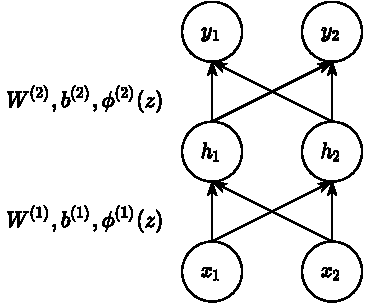
\includegraphics[width=0.3 \textwidth]{figures/q1.1.pdf}
        \end{center}
        
        \noindent Please specify the weights and activation functions for your network.
        Your answer should include: 
        \begin{itemize}
            \item Two weight matrices: $\weightMatL{1}$, $\weightMatL{2} \in \mathbb{R}^{2 \times 2}$
            \item Two bias vector: $\biasesL{1}$, $\biasesL{2} \in \mathbb{R}^{2}$ 
            \item Two activation functions: $\phi^{(1)}(z)$, $\phi^{(2)}(z)$
        \end{itemize}
        You do not need to show your work. \\
        
        \noindent \emph{Hint: Sorting two numbers is equivalent to finding the min and max of two numbers.} \\
        $$\max(x_1,x_2) = \frac{1}{2}(x_1+x_2)+\frac{1}{2}|x_1-x_2|,\qquad \min(x_1,x_2) = \frac{1}{2}(x_1+x_2)-\frac{1}{2}|x_1-x_2|$$
        
    
    \subsection{Perform Sort {\color{blue}[8 points]}}\label{sec:perform_sort}
        Draw a computation graph to show how to implement a sorting function $\hat{f}:\R^4 \to \R^4$ where $\hat{f}(x_1, x_2, x_3, x_4) = (\hat{x}_1, \hat{x}_2, \hat{x}_3, \hat{x}_4)$ and $(\hat{x}_1, \hat{x}_2, \hat{x}_3, \hat{x}_4)$ is $(x_1, x_2, x_3, x_4)$ in sorted order.
        Let us assume $\hat{x}_1 \leq \hat{x}_2 \leq \hat{x}_3 \leq \hat{x}_4$ and $x_1, x_2, x_3, x_4$ are positive and distinct. Implement $\hat{f}$ using your favourite sorting algorithms (e.g. Bubble Sort, Merge Sort). Let us denote the ``Sort\_2" module as $S$, please complete the following computation graph. Your answer does not need to give the label for intermediate nodes, but make sure to index the ``Sort\_2" module.
        
        \begin{center}
            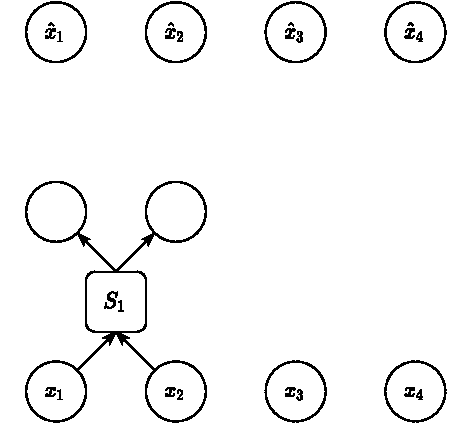
\includegraphics[width=0.3 \textwidth]{figures/q1.2.pdf}
        \end{center}
        
        \noindent \emph{Hint: Bubble Sort needs 6 ``Sort\_2" blocks, while Merge Sort needs 5 ``Sort\_2" blocks.}
    
    
    \subsection{Find the $k^{th}$ smallest number {[not graded but recommended, 0 points]}}
    Based on your sorting network, you may want to add a new layer to output your final result ($k^{th}$ smallest number). Please give the weight $\weightMatL{3}$ for this output layer when $k=3$. \\
    
    \noindent \emph{Hint: $\weightMatL{3} \in \mathbb{R}^{1 \times 4}$ .}

    \subsection{Counting Network {[not graded but recommended, 0 points]}}
    The idea of using a counting network to find the $k^{th}$ smallest number is to build a neural network that can determine the rank of each number and output the number with the correct rank. 
    Specifically, the counting network will count how many elements in a list are less than a value of interest. And you will apply the counting network to all numbers in the given list to determine their rank. Finally, you will use another layer to output the number with the correct rank.
    
    \noindent The counting network has the following architecture, where $y$ is the rank of $x_1$ in a list containing $x_1, x_2, x_3, x_4$. 
        \begin{center}
            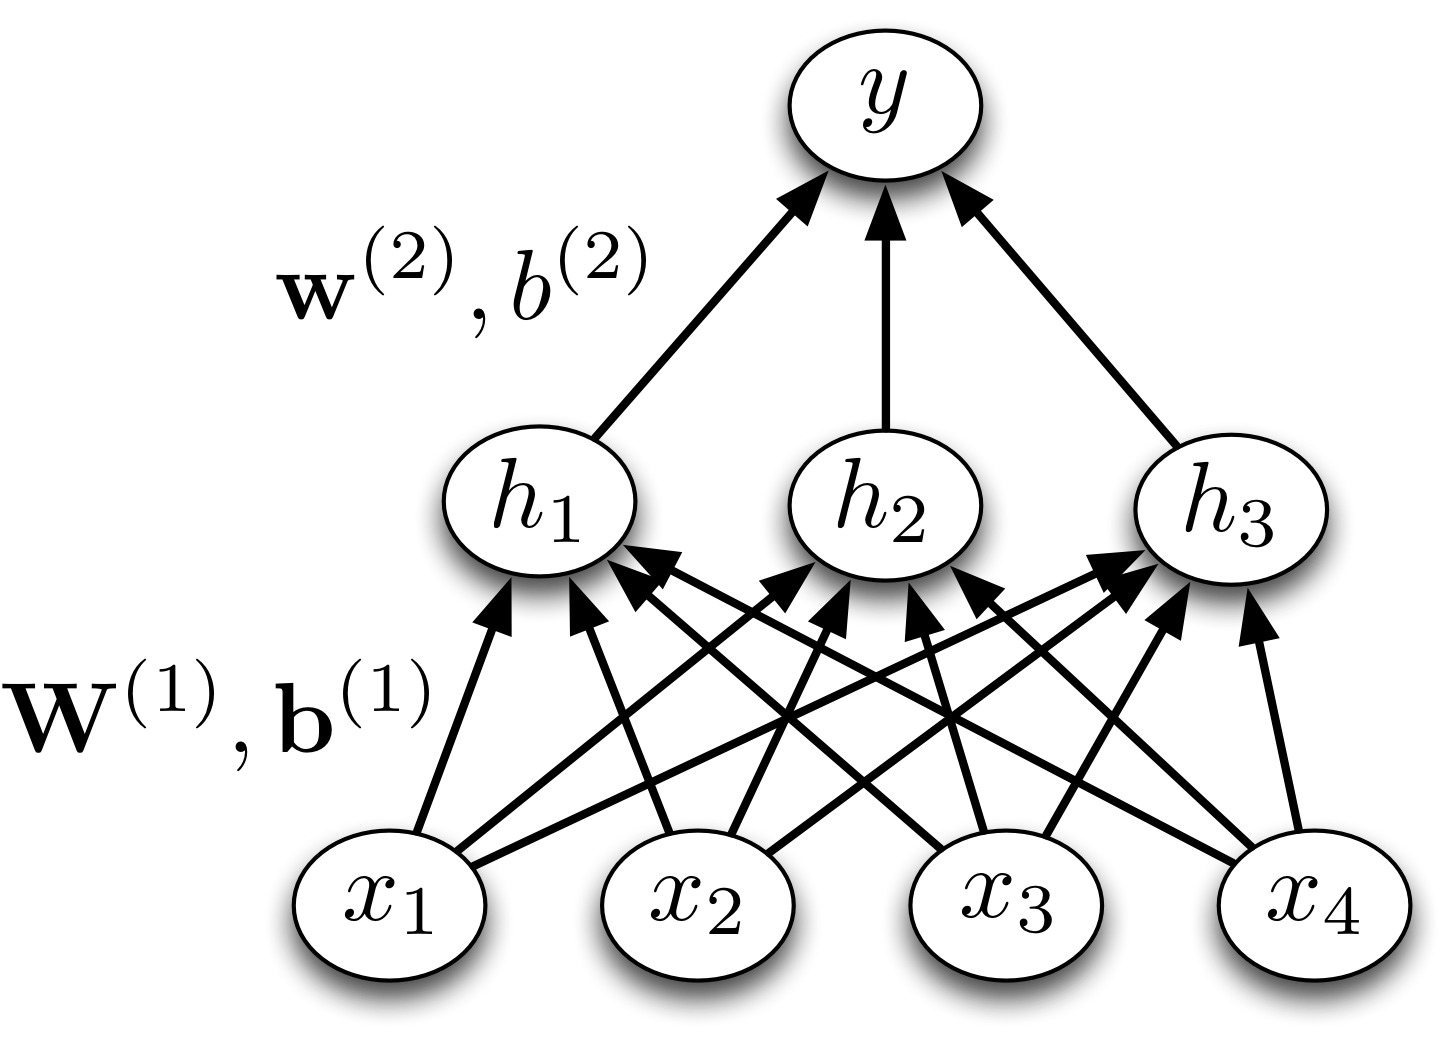
\includegraphics[width=0.3 \textwidth]{figures/architecture.png} 
        \end{center} 
        
    \noindent Please specify the weights and activation functions for your counting network. Draw a diagram to show how you will use the counting network and give a set of weights and biases for the final layer to find the $k^{th}$ smallest number. In other words, repeat the process of sections 1.1, 1.2, 1.3 using the counting idea. \\
    
    \noindent \emph{Hint: You may find the following two activation functions useful.} \\
    \noindent \emph{1) Hard threshold activation function:}
        \[ \phi(z) = \indicator(z \geq 0) = \left\{ \begin{array}{ll} 1 & \textrm{if } z \geq 0 \\ 0 & \textrm{if } z < 0 \end{array} \right. \]
    \emph{2) Indicator activation function:}
        \[ \phi(z) = \indicator(z \in [-1, 1]) = \left\{ \begin{array}{ll} 1 & \textrm{if } z \in [-1, 1] \\ 0 & \textrm{otherwise} \end{array} \right. \]
        
  
\bigskip
    
\end{document}
